\chapter{Introduction}
\label{chp:introduction}

% Performance evaluation of software architectures:  http://dl.acm.org/citation.cfm?id=287353

% Experience with Performance Testing of Software Systems: Issues, an Approach, and Case Study: http://search.proquest.com/docview/195577700?pq-origsite=gscholar

% The Future of Software Performance Engineering: http://ieeexplore.ieee.org/xpls/abs_all.jsp?arnumber=4221619&tag=1

% Performance Regression Testing Target Prioritization via Performance Risk Analysis: http://opera.ucsd.edu/paper/icse14-perfscope.pdf

% 

Performance is a make-or-break quality for software.
The cost of a software product is determined more by how well it achieves its objectives for quality attributes such as performance than by its functionality \cite{smith2003software}.

Performance can be divided in two dimensions: responsiveness and scalability.
Responsiveness is the ability of a system to meet the requirements for response time or throughput.
It can be measured by how fast a system can respond to an event or how many events can be processed in a set amount of time.
Scalability is the ability of a system to meet the required response time or throughput when faced with a growing demand of its software functions.

Performance plays an important role in both industrial and academic areas.
For instance, an increase of 500 milliseconds latency in Google's search results could cause 20\% traffic loss \cite{mayer2009search}.  
The deterioration of performance introduced by changes is often referred to as \emph{performance regression}.
Performance regression can lead to several undesired consequences such as damaged customer relationships which in turn can be the result of software not meeting its required performance.
Huang et al. provide the example of an e-commerce website that saw an increase of 2000\% in their page loading times because of an update to the underlying database engine \cite{huang2014performance}.
These situations can lead to lost revenue and possibly missed market windows.
Other consequences of performance failures may express themselves in lost productivity for users, increased costs, failures on deployment or even abandonment of projects \cite{woodside2007future, williams1998performance}.

To inspect whether the performance of a system has decreased, performance regression testing can be applied.
Using this method, the system is tested for performance regression under various loads \cite{woodside2007future}.
Traditional software development focusses on correctness, causing regression testing to be deferred to a late stage in the development cycle, if applied at all.
%This approach is often called the \enquote{fix-it-later} approach.
To illustrate the varying amounts of regression testing appliances, Huang et al. mention the performing testing interval of MySQL, Linux and Chrome.
These projects apply performance tests every release, every week and every four revisions, respectively.
Once performance regression is detected, developers have to spend extra efforts determining what causes said regression, especially when a lot of changes have been applied since the last measurement \cite{huang2014performance}.
Performance tests should be executed as frequently as possible, ideally per change made by developers.
However, as some tests take hours or even weeks, this approach is not always feasible.

\emph{Software performance engineering} (SPE) is the discipline concerned with constructing software systems that meet performance objectives \cite{smith2003best}.
It prescribes principles for creating responsive software, methods to to obtain performance specifications and offers guidelines for the types of evaluations to be conducted at each development stage.
SPE features two general approaches \cite{woodside2007future} where the first approach is purely measurement based.
This characterizes itself by performing actions late in the development cycle such as  applying regression tests, diagnosis and tuning, when the system can be run and measured in real-time.
The second approach features a model-based style.
Using this approach, performance models are created at the early stages of development, influencing the architecture and design of the system to meet performance requirements.

\todo{Uitleggen dat performance in centralized architecturen makkelijker is te tunen dan een decentraal systeem + plaatje met verschil}.

\begin{figure}[!h]
	\centering
	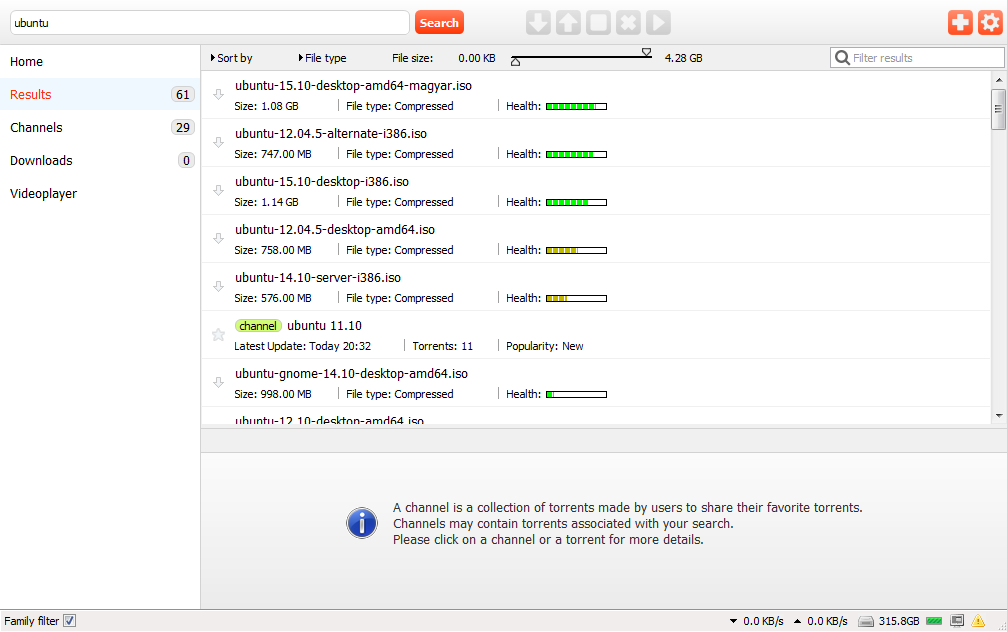
\includegraphics[width=\linewidth]{introduction/images/tribler_screenshot.png}
	\caption{Screenshot of Tribler v6.5.2.}
	\label{fig:tribler_screenshot}
\end{figure}

Tribler is the result of ten years of scientific research in the field of decentralized networks and online cooperation.
Over 100 scientific publications have Tribler in their foundation.
Tribler is completely open-source and can be downloaded from the Tribler website\footnote{\url{https://www.tribler.org}}.
Over the course of more than a decade Tribler has gained a tremendous amount of attention in both media and academia.
It has been downloaded approximately 1.8 million times and has more than two thousand \todo{cite to support this} monthly active users.
This makes Tribler one of the research projects that allow researchers to run experimental code \enquote{in the wild} on a large scale.

One of Tribler's unique features is that it allows users to discover and exchange data in a complete decentralized way.

To offer privacy and anonymity, support for anonymous downloads were introduced in 2014 by R. Plak \cite{plak2014anonymous} and R. Tanaskoski \cite{tanaskoski2014anonymous}.
In 2015, the support for anonymous seeding of torrents using Tor-like hidden services was added by R. Ruigrok \cite{ruigrok2015bittorrent}.
A trade-off has to be made by Tribler between the desired performance and the level of anonymity provided, as any additional layer of privacy comes with an increased number of cryptographic operations.

Not only anonymity impacts the overall performance of Tribler: architectural flaws introduced in the past have led to a decrease in performance today.
This manifests itself in users frequently reporting high system load, a non-responsive Graphical User Interface (GUI) and low download speed.
Furthermore, Tribler is plagued with a high number of disk operations which has been known since 2013 \cite{pouwelse2014reduce}. 
Its interface visible in Figure~\ref{fig:tribler_screenshot}.

The focus of this thesis is to improve Tribler's performance by making use of software performance engineering techniques with a particular focus on the performance of disk operations and software regression testing.

The rest of this thesis is structured as follows.
Chapter~\ref{chp:problem-description} provides the problem description and the research questions this thesis attempts to answer.
Chapter~\ref{cpt:related_work} presents related work on the subjects overlapping this thesis work.
Chapter~\ref{cpt:pythons_thread_model} explains the python threading module and why parallel programming in Python is different from a language such as Java. Additionally, the subjects of multi-threaded performance and asynchrony are covered.
Chapter~\ref{implementation_and_experiments} presents the implementation details and experimental results of this work.
Finally, Chapter~\ref{cpt:conclusion_and_future_work} concludes this thesis and provides future work.

\section{old text}
Experiments are at the hearth of science.
This understanding was introduced by Sir Isaac Newton in his revolutionary work \emph{hilosophiae naturalis principia mathematica}.
Newton reasoned that researchers are to test their hypothesis with observable, measurable and empirical experiments.
To this day, this approach is applied by many researchers.

Especially in the area of Computer Science, it is key to provide empirical proof that a hypothesis one ought to prove holds.
This empirical proof often manifests itself in the form of benchmarking.
By benchmarking several programs/algorithms or different versions of the same program/algorithm on a variety of workloads, one can observe if there are notable changes in predefined metrics such as time or memory consumption.

Over the course of years, profilers have been introduced to allow developers to profile their running code.
By inspecting the data generated by these profilers, developers can pinpoint functions that are consuming e.g. a lot of time which may indicate a bottleneck is present.
Additionally, once a bottleneck has been resolved it can be verified by using a profiler that it indeed does consume less resources, i.e. time or memory.

In large and complex systems there are likely to be many bottlenecks present.
J. M. Juran's Pareto principle admonishes that one should "Concentrate on the vital few, not the trivial many" \cite{ammons2004finding}. This principle is also known as the 80/20 rule.
Concretely, this means that resolving the vital bottlenecks yields the best diminishing returns.
This principle holds even for large systems.

In this thesis we use the BitTorrent client Tribler as a use case to implement a regression testing system and to find and resolve bottlenecks, demonstrating the working of said system.
Tribler has been in development for over ten years and has grown into a highly complex and large distributed system.
Along with its components, it features more than 158 KLOC \cite{tribler2015about}.
Currently, the adoption of Tribler is hampered by its performance. 
Products such as YouTube, FaceBook and Wikipedia have millions or even billions of monthly active users.
Here, speed plays a key role: an increase of 500ms latency could reduce Google's traffic by 20\% \cite{mayer2009search}.

\section{Tribler}

Tribler is a research platform for self organizing systems and online cooperation.
All research is embedded in the Tribler BitTorrent client, visible in Figure~\ref{fig:tribler_screenshot}.
Tribler can be downloaded free of charge from the Tribler website\footnote{\url{https://www.tribler.org}}.
It has been downloaded approximately 1.8 million times, has more than 2 thousand monthly active users and anticipating more growth in the near future.
This makes Tribler one of the few research projects that allow researchers to run experimental code \enquote{in the wild} on a large heterogeneous user group.

Tribler focuses on the following goals:
\begin{itemize}
    \item Allow for secure and private communication and sharing of data.
    \item Enforce user contribution in the network by making use of the Multi-Chain.
    \item Reward seeding of poorly-seeded content by using credit mining.
    \item Make it impossible to shut Tribler down, unless the Internet itself as a whole gets taken down.
\end{itemize}

A fully decentralized ecosystem i.e. no central components present, is Tribler's approach to achieve these goals.
Tribler has been designed and build with this focus~\cite{Pouwelse-tribler,Bakker-tribler} \todo{cites}.
A distributed network requires both the presence and collaboration of participants, called peers, to be able to achieve this.

\section{Dispersy}
The Distributed Permission System (Dispersy) is an elastic database system written in the Python programming language and uses SQLite as its underlying database engine.

\subsection{Challenging network conditions}
Nowadays almost all devices have an internet connection, often running in a challenged network environment \cite{dispersy2016dispersy}.
Challenging conditions can be found in many different networks such as Peer-to-Peer (P2P) networks or delay tolerant networks (DTNs).
The limitations of these networks are often low internet speed, connection drops, package loss and long communication delays.
P2P networks in particular create challenging conditions as many devices are not online at all times, they are often behind NAT-firewall constrained internet connections and one often interacts with byzantine peers.
Additionally, smartphones and other embedded devices such as Raspberry PI's often have less processing capacity or finite battery lifetime.

Dispersy is designed to still function when faced with these challenging network conditions.
It does this by using optimized algorithms, protocols and other techniques such as bloom filters to minimize the amount of resources needed.
By making use of strong elliptic curve cryptography, nodes are identified in a secure and anonymous way.

\subsection{Decentralized}
Dispersy is fully decentralized with the exception of bootstrap servers.
It can run on systems with a large number of nodes, without any sever architecture needed.
All nodes perform the same algorithmic procedures and tasks and do not differentiate between any node i.e. all nodes are equal.

Furthermore, Dispersy provides on-to-one and one-to-many data dissemination mechanisms to forward data to nodes.
Eventually, all data will reach all nodes in the network, overcoming challenging network conditions.

\section{BitTorrent protocol}
The BitTorrent protocol was introduced in 2001 and been a huge part of the internet ever since \cite{Cohen2001BitTorrent}.
Estimates as of 2009 indicate that 43\% to 70\% of all internet traffic world-wide is caused by peer-to-peer networks \cite{schulze2009internet}.
As of February 2013, BitTorrent was responsible for 3.35\% of all worldwide bandwidth \cite{palo2013application}, having 15 - 27 million concurrent users at any time \cite{wang2013measuring} and more than 150 million users in total \cite{reuters2012bittorrent}.

Downloading files is done in a decentralized way, that means no central entity such as a server is needed.
By obtaining a torrent file, users can download files associated with this torrent using a program that is compatible with the BitTorrent protocol.\\

A torrent is a file that contains meta information about the directories and files to be distributed.
More specifically, it contains names, sizes, hashes to verify the integrity of the files and the folder structure of the content to be downloaded.
A torrent usually contains a list of trackers and their network addresses.
These trackers help participants locate each other and form efficient distribution groups -- \emph{swarms}.
 

When sharing files by using the BitTorrent protocol, a user (or peer) that uploads i.e. allows other peers to download the user's files using the user's upload connection, is called a seeder.
A peer that is downloading a file of a seeder is called a leecher.
Any peer can be both a seeder and leecher at the same time, and join the network at any given time.\\

The ratio between the total data downloaded and uploaded is called the seeding ratio \cite{Cohen-bittorrent}.
The seeding ratio can be seen as an indication of the level of collaboration i.e. giving back resources to the network.\\

%Seeding can be seen as an interaction between peers, where the seeder aids the leeching peer.
%By utilizing the seeders upload bandwidth, the leeching peer can use his download bandwidth to download a file.
%While there is a clear incentive for the leecher by downloading the desired file, there is none for the seeder.
%Especially since the leecher has a little chance of becoming also be a seeder for the original seeder \cite{Lai-Incentives}.\\

%Having peers actively and persistently contribute to the network will increase the network's health which in turn provides several benefits for all peers.
%A more healthy network results in a higher availability of seeders and results in high download speeds.
%It has been shown that private communities i.e. "darknets" where the seeding ratio is high, provides better download conditions \cite{meulpolder-privatecommunities}.
%In these private communities, trackers i.e. central components introduce peers to each other using the Tit-for-tat approach \cite{cohen-titfortat}.
%The Tit-for-Tat approach is aiding peers who have aided you in the past,
%The absence of trackers, which is often the case in public networks, results in free-riding \cite{Adar-Freeriding}.
%A free-riding peer does not or gives little back to the network while receiving all benefits i.e. download without any restriction.
%\todo{Explain the optimistic chocking approach.}
%BitTorrent applies a variation of the Tit-for-tat strategy, optimistic chocking, to combat this problem.
%The Tit-for-Tat strategy is to only provide help to peers that return this help.
%However, it has been shown that this approach is not effective in battling abuse \cite{Pouwelse-tribler}.


\todo{more explanation?}
\section{Goal \& Outline}
In this thesis we introduce a performance regression testing system that makes use of benchmarking.
Whenever a codebase changes, it is important to measure the effects of these changes.
Negative changes can manifest themselves as reduced computational speed, increased memory consumption or reduced responsiveness of a program.
Each of these result in a reduction of user experience.
For instance, Google Chrome makes use of performance regression testing to gain insight into the effect of code changes.
While it is one of the fastest browsers currently available, it is also know for it's extreme RAM consumption which may lead to issues on older devices \cite{ram2012chrome}.

In this chapter we provided an introduction of this thesis and presented the research questions this thesis aims to answer. 
This section describes the other chapters in this thesis.
Chapter~\ref{chp:problem-description} provides the problem description and the research questions this thesis attempts to answer.
Chapter~\ref{cpt:related_work} presents related work on the subjects overlapping this thesis work.
Chapter~\ref{cpt:pythons_thread_model} explains the python threading module and why parallel programming in Python is different from a language such as Java. Additionally, the subjects of multi-threaded performance and asynchrony are covered.
Chapter~\ref{implementation_and_experiments} presents the implementation details and experimental results of this work.
Finally, Chapter~\ref{cpt:conclusion_and_future_work} concludes this thesis and provides future work.
